\begin{figure}[htbp]

\begin{center}
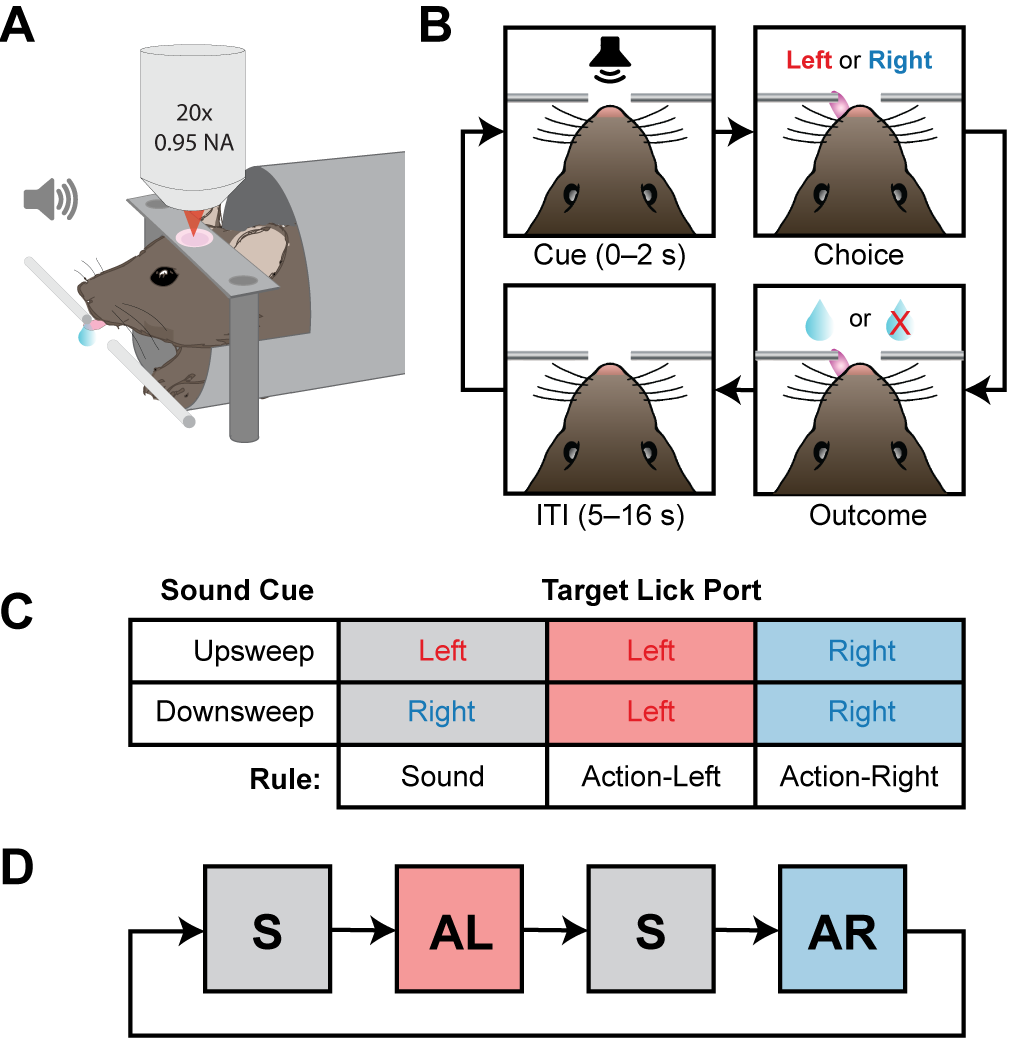
\includegraphics[width=8.7cm]{Figures/Fig1.png} 
\end{center}

\caption[Rule switching task for head-fixed mice.]
{Rule switching task for head fixed mice. (A) Experimental setup for two-choice sensorimotor task with simultaneous two-photon imaging. Mice rested inside of a stainless steel tube, with the head immobilized using a cranial implant. Two lick ports were placed on either side of the mouth to deliver water rewards. (B) Flow diagram of trial structure. A sound cue was played at the start of each trial, indicating the target port that would be rewarded (left or right). To obtain the reward, subjects were required to lick the target within 2 s following cue onset. After a random intertrial interval (ITI) of 5--16 s, a new sound cue was presented, providing a fresh opportunity to lick for a reward. (C) Table indicating the target lick port signified by each sound cue in each rule context. (D) Flow diagram of session structure. Trials governed by each rule were organized into blocks. Sound blocks (S) were interleaved with action blocks that alternated between the action-left (AL) and action-right (AR) rule. A new rule block was initiated on the next trial after an accuracy criterion was met (85\% for the past 20 trials of the current block).}

\label{fig:Fig1}
\end{figure}